% Template for Cogsci submission with R Markdown

% Stuff changed from original Markdown PLOS Template
\documentclass[10pt, letterpaper]{article}

\usepackage{cogsci}
\usepackage{pslatex}
\usepackage{float}
\usepackage{caption}

% amsmath package, useful for mathematical formulas
\usepackage{amsmath}

% amssymb package, useful for mathematical symbols
\usepackage{amssymb}

% hyperref package, useful for hyperlinks
\usepackage{hyperref}

% graphicx package, useful for including eps and pdf graphics
% include graphics with the command \includegraphics
\usepackage{graphicx}

% Sweave(-like)
\usepackage{fancyvrb}
\DefineVerbatimEnvironment{Sinput}{Verbatim}{fontshape=sl}
\DefineVerbatimEnvironment{Soutput}{Verbatim}{}
\DefineVerbatimEnvironment{Scode}{Verbatim}{fontshape=sl}
\newenvironment{Schunk}{}{}
\DefineVerbatimEnvironment{Code}{Verbatim}{}
\DefineVerbatimEnvironment{CodeInput}{Verbatim}{fontshape=sl}
\DefineVerbatimEnvironment{CodeOutput}{Verbatim}{}
\newenvironment{CodeChunk}{}{}

% cite package, to clean up citations in the main text. Do not remove.
\usepackage{cite}

\usepackage{color}

% Use doublespacing - comment out for single spacing
%\usepackage{setspace}
%\doublespacing


% % Text layout
% \topmargin 0.0cm
% \oddsidemargin 0.5cm
% \evensidemargin 0.5cm
% \textwidth 16cm
% \textheight 21cm

\title{A Language's Unigram Entropy Distribution Predicts Self-Paced Reading
Times}


\author{{\large \bf Josef Klafka} \\ \texttt{jklafka@uchicago.edu} \\ Department of Psychology \\ University of Chicago \And {\large \bf Daniel Yurovsky} \\ \texttt{yurovsky@uchicago.edu} \\ Department of Psychology \\ University of Chicago}

\begin{document}

\maketitle

\begin{abstract}
We provide evidence against the Uniform Information Density (Jaeger,
2010) and wrap-up effect hypotheses.

\textbf{Keywords:}
Entropy; self-paced reading; information theory; language processing
\end{abstract}

\section{Uniform Information Density}\label{uniform-information-density}

A major line of research in the current century has asked how speakers
and writers distribute information in the linguistic material they
produce. This begins with Claude Shannon in the years after World War
II. Shannon (1948) defined ``information'' as a ``reduction in
uncertainty''. Shannon followed by quantifying uncertainty in his
measure of \emph{entropy}: the amount of uncertainty on the outcome of a
random variable. Shannon proposed that the most efficient method of
sending information through a noisy channel is at a constant rate.
Genzel \& Charniak (2002) apply this principle to human communication:
if people communicate information through speech and text optimally,
then we should transmit information to one another at a constant rate.
Genzel \& Charniak created a distribution of estimates for
sentence-level entropy, each sentence taken without context, for
newspaper articles from the Penn Treebank corpus. Obtaining a roughly
monotonically increasing linear distribution, Genzel \& Charniak
proposed the \emph{Constant Entropy Rate} (CER) principle: the entropy
rate in speech and text with context should be constant as sentence
number increases. Aylett \& Turk (2004) proposed a similar principle for
the phonological level.

Jaeger (2010) extends the CER principle to all levels of human
communication: the \emph{Uniform Information Density} (UID) hypothesis.
Jaeger argues that speakers will try to distribute information more
evenly over the course of an utterance, to be as close to channel
capacity (in a Shannon sense) as possible. In particular, Jaeger singles
out the production of ``that'' at the beginning of relative clauses in
English and the use of contractions such as ``he's'' and ``you're''
versus ``he is'' and ``you are'' as instances where higher information
density in the clause elicits the production of more material by
speakers.

The \emph{wrap-up effect} is a popular hypothesis within the
eye-tracking community. The hypothesis states that, in written text,
sentence-final words are processed more slowly on average then
sentence-medial or sentence-initial words, due to readers integrating
information from the entire sentence in order to form a final, coherent
thought expressed by the sentence, among other reasons. With these two
ideas, information production distribution in spoken and written
communication, and information integration in reading written texts, we
move on to discuss cross-linguistic differences in the distribution of
information across sentences.

The UID hypothesis

\subsection{UID challenges}\label{uid-challenges}

More recent work has stood out in contrast to the traditional UID
perspective. Zhan and Levy (2018) study Mandarin Chinese classifier use,
and find that the use of specific classifier, versus general
classifiers, appears more often in cases where the production of the
corresponding noun is more difficult than when the production is easier,
as would be predicted by UID. The UID perspective is challenged in Yu et
al. (2016), by performing an analysis of entropy by position in the text
portion of the British National Corpus. They use the following formula
for each word position X of sentences of fixed length k from the corpus,
where each i is a word occurring in position X and pi is the number of
times word i occurs in position X divided by the number of total words
that occur in position X i.e.~the number of sentences of length k.

\[H(X) = \sum\limits_w p(w)\log\big(p(w)\big)\] Yu et al. (2016) refer
to their distribution for English as a `three-step distribution':
relatively low entropy at the beginning of a sentence, then a jump, then
flat entropy in the middle, a dip before the final position and a jump
with the final word. View the figure below for a visual demonstration.

\begin{CodeChunk}
\begin{figure*}[h]

{\centering 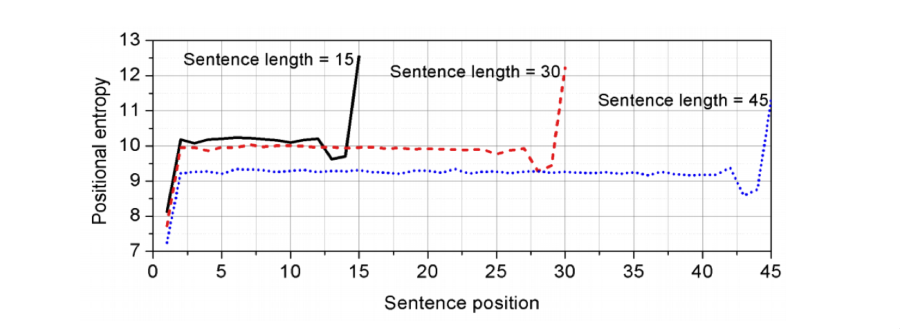
\includegraphics{figs/yunigram-1} 

}

\caption[English entropy distribution for three sentence lengths from BNC]{English entropy distribution for three sentence lengths from BNC}\label{fig:yunigram}
\end{figure*}
\end{CodeChunk}

\section{Our Methods}\label{our-methods}

We used the CHILDES TalkBank (Brown 1973; MacWhinney 2000) corpora
database of spoken adult-child conversations. We first used the Brown
and Providence English corpora from CHILDES. The Brown corpus contains
conversations between three young children (over 1.5 years old and under
6 years old) and their families in the home. The Providence corpus
contains transcriptions of audio/video files which recorded interactions
between children between 1 and 3 years old and their parents in the
home.

\begin{CodeChunk}
\begin{figure*}[h]

{\centering 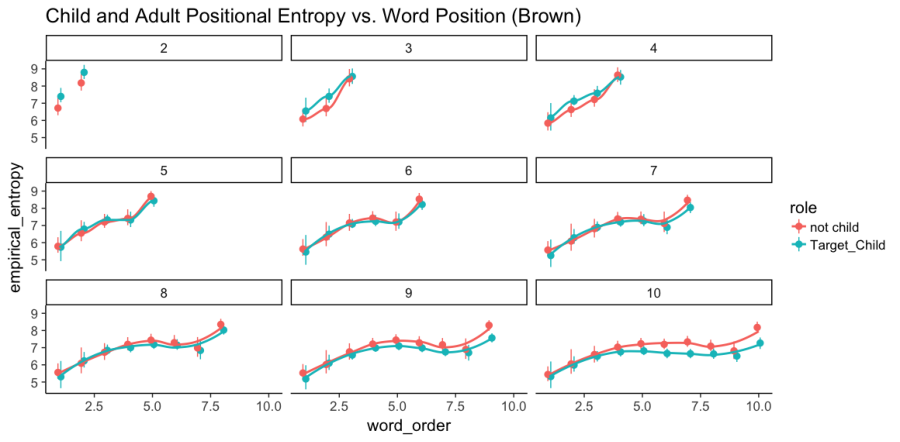
\includegraphics{figs/brown_PE-1} 

}

\caption[Brown corpus entropy]{Brown corpus entropy}\label{fig:brown_PE}
\end{figure*}
\end{CodeChunk}

\begin{CodeChunk}
\begin{figure*}[h]

{\centering 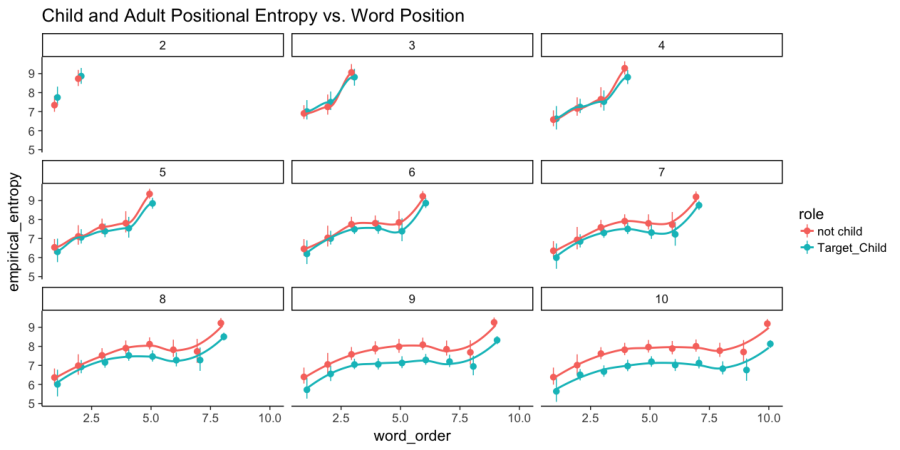
\includegraphics{figs/providence_PE-1} 

}

\caption[Providence corpus unigram entropy]{Providence corpus unigram entropy}\label{fig:providence_PE}
\end{figure*}
\end{CodeChunk}

We found a similar distribution for Spanish and German corpora from
CHILDES. The Spanish corpus we used was the XXX and the German corpus we
used was the XXX.

\section{Formalities, Footnotes, and
Floats}\label{formalities-footnotes-and-floats}

Use standard APA citation format. Citations within the text should
include the author's last name and year. If the authors' names are
included in the sentence, place only the year in parentheses, as in
(1972), but otherwise place the entire reference in parentheses with the
authors and year separated by a comma (Newell \& Simon, 1972). List
multiple references alphabetically and separate them by semicolons
(Chalnick \& Billman, 1988; Newell \& Simon, 1972). Use the et. al.
construction only after listing all the authors to a publication in an
earlier reference and for citations with four or more authors.

For more information on citations in RMarkdown, see
\textbf{\href{http://rmarkdown.rstudio.com/authoring_bibliographies_and_citations.html\#citations}{here}.}

\subsection{Footnotes}\label{footnotes}

Indicate footnotes with a number\footnote{Sample of the first
footnote.} in the text. Place the footnotes in 9 point type at the
bottom of the page on which they appear. Precede the footnote with a
horizontal rule.\footnote{Sample of the second footnote.} You can also
use markdown formatting to include footnotes using this
syntax.\footnote{Sample of a markdown footnote.}

\subsection{Figures}\label{figures}

All artwork must be very dark for purposes of reproduction and should
not be hand drawn. Number figures sequentially, placing the figure
number and caption, in 10 point, after the figure with one line space
above the caption and one line space below it. If necessary, leave extra
white space at the bottom of the page to avoid splitting the figure and
figure caption. You may float figures to the top or bottom of a column,
or set wide figures across both columns.

\subsection{Two-column images}\label{two-column-images}

You can read local images using png package for example and plot it like
a regular plot using grid.raster from the grid package. With this method
you have full control of the size of your image. \textbf{Note: Image
must be in .png file format for the readPNG function to work.}

You might want to display a wide figure across both columns. To do this,
you change the \texttt{fig.env} chunk option to \texttt{figure*}. To
align the image in the center of the page, set \texttt{fig.align} option
to \texttt{center}. To format the width of your caption text, you set
the \texttt{num.cols.cap} option to \texttt{2}.

\begin{CodeChunk}
\begin{figure*}[h]

{\centering 
\includegraphics{figs/2-col-image-1} 

}

\caption[This image spans both columns]{This image spans both columns. And the caption text is limited to 0.8 of the width of the document.}\label{fig:2-col-image}
\end{figure*}
\end{CodeChunk}

\subsection{One-column images}\label{one-column-images}

Single column is the default option, but if you want set it explicitly,
set \texttt{fig.env} to \texttt{figure}. Notice that the
\texttt{num.cols} option for the caption width is set to \texttt{1}.

\begin{CodeChunk}
\begin{figure}[H]

{\centering 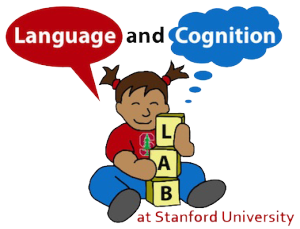
\includegraphics{figs/image-1} 

}

\caption[One column image]{One column image.}\label{fig:image}
\end{figure}
\end{CodeChunk}

\subsection{R Plots}\label{r-plots}

You can use R chunks directly to plot graphs. And you can use latex
floats in the fig.pos chunk option to have more control over the
location of your plot on the page. For more information on latex
placement specifiers see
\textbf{\href{https://en.wikibooks.org/wiki/LaTeX/Floats,_Figures_and_Captions}{here}}

\begin{CodeChunk}
\begin{figure}[H]

{\centering 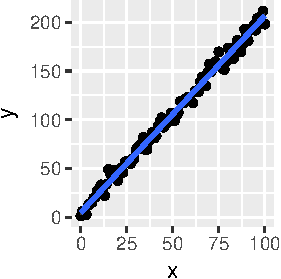
\includegraphics{figs/plot-1} 

}

\caption[R plot]{R plot}\label{fig:plot}
\end{figure}
\end{CodeChunk}

\subsection{Tables}\label{tables}

Number tables consecutively; place the table number and title (in 10
point) above the table with one line space above the caption and one
line space below it, as in Table 1. You may float tables to the top or
bottom of a column, set wide tables across both columns.

You can use the xtable function in the xtable package.

\begin{table}[H]
\centering
\begin{tabular}{rrrrr}
  \hline
 & Estimate & Std. Error & t value & Pr($>$$|$t$|$) \\ 
  \hline
(Intercept) & -0.10 & 0.11 & -0.9 & 0.37 \\ 
  x & 1.97 & 0.12 & 16.6 & 0.00 \\ 
   \hline
\end{tabular}
\caption{This table prints across one column.} 
\end{table}

\section{Acknowledgements}\label{acknowledgements}

Place acknowledgments (including funding information) in a section at
the end of the paper.

\section{References}\label{references}

\setlength{\parindent}{-0.1in} \setlength{\leftskip}{0.125in} \noindent

\hypertarget{refs}{}
\hypertarget{ref-ChalnickBillman1988a}{}
Chalnick, A., \& Billman, D. (1988). Unsupervised learning of
correlational structure. In \emph{Proceedings of the tenth annual
conference of the cognitive science society} (pp. 510--516). Hillsdale,
NJ: Lawrence Erlbaum Associates.

\hypertarget{ref-NewellSimon1972a}{}
Newell, A., \& Simon, H. A. (1972). \emph{Human problem solving}.
Englewood Cliffs, NJ: Prentice-Hall.

\end{document}
